\documentclass[conference]{IEEEtran}
\IEEEoverridecommandlockouts
% The preceding line is only needed to identify funding in the first footnote. If that is unneeded, please comment it out. \usepackage{cite} \usepackage{amsmath,amssymb,amsfonts}
\usepackage{algorithmic}
\usepackage{graphicx}
\usepackage{tabularx}
\usepackage{textcomp}
\usepackage{fancyvrb}
\usepackage{wrapfig}
\usepackage{xcolor}
\usepackage{xspace}
\usepackage{multirow}
\usepackage{longtable}
\usepackage{listings}

\usepackage{pifont}
\def\BibTeX{{\rm B\kern-.05em{\sc i\kern-.025em b}\kern-.08em
    T\kern-.1667em\lower.7ex\hbox{E}\kern-.125emX}}
    
\newcommand*{\lorawan}{LoRaWAN\xspace}
\newcommand*{\iic}{I$^2$C\xspace}
\newcommand*{\kOhm}{k$\Omega$\xspace}


\begin{document}

\section*{}
\begin{center}
{\huge Aether Sensor Network} \\ \vspace{2 em}
{\Large Ian Wallace, Paul Wood, Randy Alvarez, Parke Benjamin} \\ \vspace{2em}
{\Large College of Electrical and Computer Engineering, University of Central Florida, Orlando, FL, 32826, USA} \\ \vspace{3em}
\end{center}


\begin{abstract}
Poor or even hazardous air quality can pose a health risk to those with respiratory conditions or those in vulnerable age groups, such as the elderly and young children. Therefore the ability to monitor the local air quality is vital. In this paper, we present our design for a low power, air quality monitoring system called Aether. Aether uses gas and particulate matter sensors to collect the data used in calculating air quality. This data is sent over a LoRaWAN network to a server where the air quality index is computed. The data is then displayed on a web page for viewing by the user. This includes the ability to see the different data overlaid
\end{abstract}

\begin{IEEEkeywords}
air quality index, solar power, LoRa, LoRaWAN, low power, internet of things
\end{IEEEkeywords}

\section{Introduction}
The Aether Sensor Network is a low-power, air quality monitoring system. The Aether Sensor Network consists of two main components: the device which collects air quality data, known as the Aether Node, and a web server that hosts and displays that data. The Aether Node uses multiple gas sensors to collect the data used in calculating air quality. This collected data is transmitted by the Aether Node over \lorawan, an upcoming technology that has been growing in popularity recently for use in internet of things (IoT) applications, to a server. The Aether Node is implemented on a four-layer PCB and housed in a 3D printed enclosure. The computation that is performed by the Aether Node is done by a Seeed LoRa-E5 LoRaWAN module. This module packages an ST STM32WLE5JC, which is an SoC combing an ARM M4 processor and a LoRa chip. Figure \ref{fig:overall-bd} shows how the LoRa-E5 module processes data collected from the three primary senors of the Aether Node, which include the two main gas sensors, a Renesas ZMOD4510 and a Bosch BME688, and a Sensirion SPS30 particulate matter sensor. The LoRa-E5 module transmit the collected sensor data to the second major component of the Aether Sensor Network, the web server. 

As seen in Figure \ref{fig:overall-bd}, the web server used by Aether is hosted on Amazon Web Services (AWS) and uses Supabase for the database and API. Finally, the results are results are displayed on a web page using the popular JavaScript framework, React. Through this web page, users can see map with the data collected from all Aether Nodes that have been registered with the server overlaid on an Mapbox map. Users are able to add alerts for different events, such as when the AQI exceeds a user-defined threshold. These alerts will be sent to the user through email.

\begin{figure}[b]
    \centering
    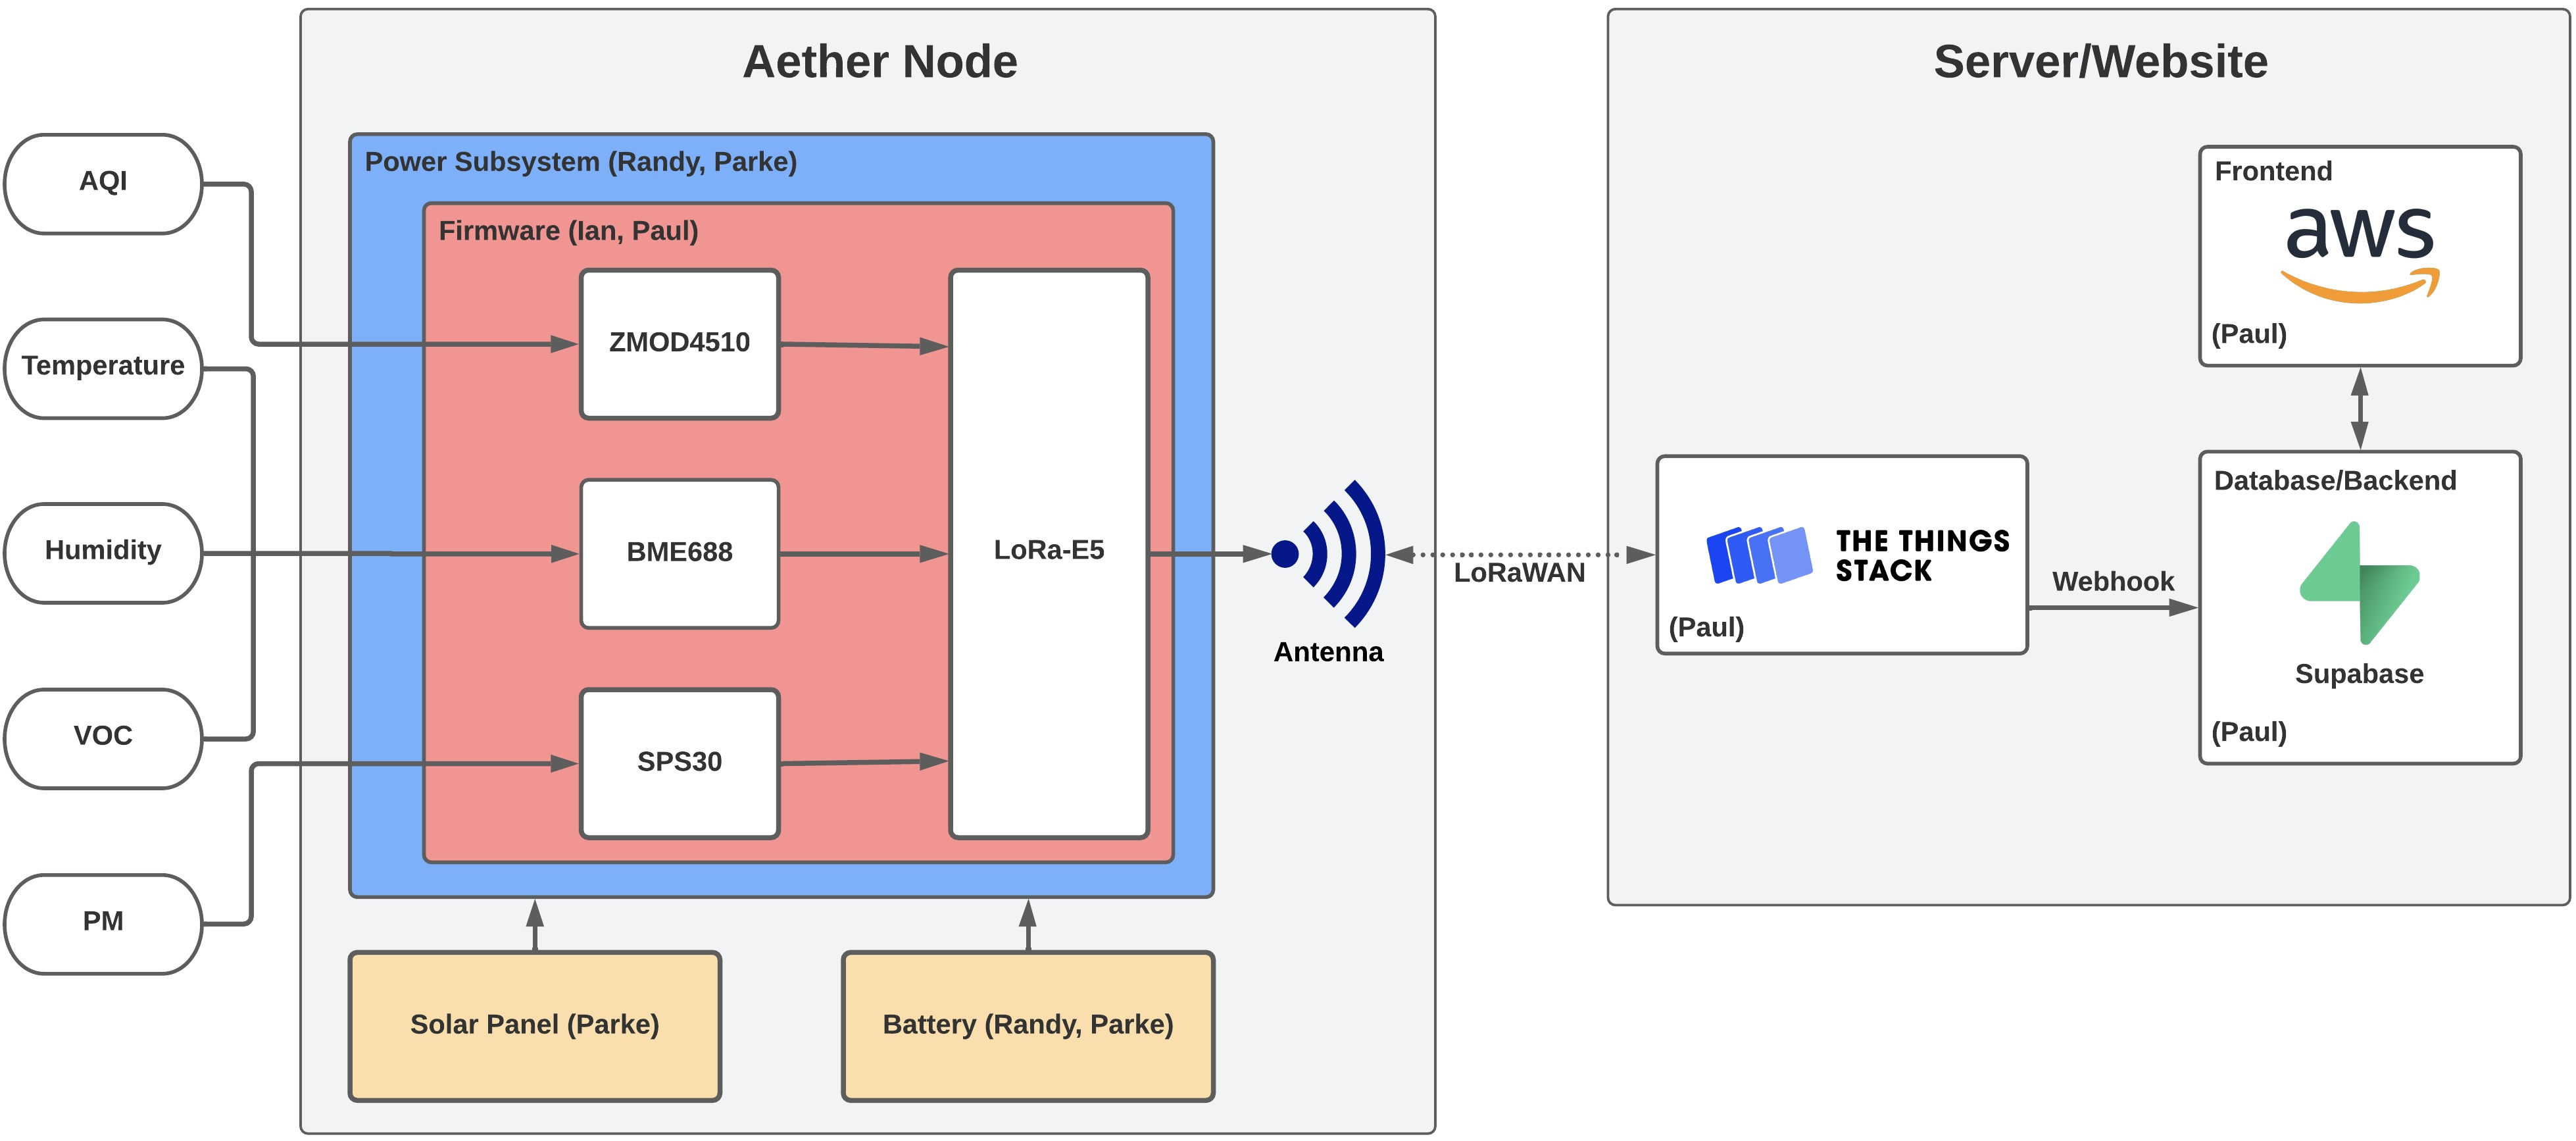
\includegraphics[width=3.3in]{img/aether-overall-bd.jpeg}
    \caption{An overall block diagram of the Aether Sensor Network.}
    \label{fig:overall-bd}
\end{figure}

\section{Background}

%\subsection{Air Quality Index}
The Air Quality Index (AQI) is a metric used by the EPA for measuring the overall air quality in an area. Table \ref{tab:aqi-levels} shows the range of AQI values and the corresponding levels of health concern. AQI can be calculated from the readings of any of the following seven measured pollutants: These include PM2.5, PM10, sulfur dioxide, nitrogen oxides, carbon monoxide, and ozone. The final AQI value is based on the maximum AQI that was calculated from each of the six pollutants. It is not required to have readings from all six pollutants in order to calculate the AQI \cite{background-aqi}. Therefore, the two primary pollutants that we will focused on measuring are particulate matter (PM2.5 and PM10) and ozone (O$_3$).

\begin{enumerate}
    \item \textbf{Particulate matter}, as defined by the EPA, is any tiny liquid or solid droplets that can be inhaled and cause serious health effects. Coarse particles (PM10) are defined as particles that are 10 um or less. Fine particles (PM2.5) are defined as particles that are 2.5 um or less \cite{background-pm}.
    \item \textbf{Ozone}, more specifically ground-level ozone, as defined by the EPA, is a highly reactive gas and is not naturally forming, unlike stratospheric ozone \cite{background-ozone}.
\end{enumerate}

%\subsection{LoRaWAN}

\begin{table}
\centering
\caption{The Different AQI Levels \cite{background-aqi}}

\begin{tabular}{|c|c|c|}
\hline
AQI Values & Level of Health Concern & Color \\\hline\hline
0-50 & Good & Green \\\hline
51-100 & Moderate & Yellow \\\hline
101-150 & Unhealthy for Sensitive Groups & Orange \\\hline
151-200 & Unhealthy & Red \\\hline
201-300 & Very Unhealthy & Purple \\\hline
301-500 & Hazardous & Maroon \\\hline
\end{tabular}

\label{tab:aqi-levels}
\end{table}


\section{System Components}
The design of Aether Node will be easier to understand if the major components in the design are explained beforehand. Therefore, before going through the design of the Aether Node, we will first provide an introduction to each of the major components in the design. 

\subsection{Sensor Hardware}
In this section, we will discuss the sensors used in the Aether Node. The Aether Node is equipped with three primary sensors:
\begin{enumerate}
\item The Bosch BME688
\item The Renesas ZMOD4510
\item The Sensirion SPS30
\end{enumerate}
The Bosch BME688 is able to measure temperature, humidity, and pressure. The sensor can also be trained, using machine learning, to recognize a particular gas. These include Volatile Organic Compounds (VOCs), volatile sulfur compounds (VSCs) and other gases such as carbon monoxide and hydrogen. However, we did not use this feature in our final design. The Renesas ZMOD4510 can measure nitrogen dioxide (NO2) and ozone (O$_3$). The SPS30 is capable of detecting both PM2.5 and PM10.

\subsubsection{Bosch BME688}
The Bosch BME688 detects volatile organic compounds (VOCs), volatile sulfuric compounds (VSCs), and other gases through the use of sophisticated machine learning algorithms. This sensor comes in a 3.0 mm x 3.0 mm x 0.93 mm metal lid 8-pin LGA. The sensor supports both I2C and SPI. For our design, we will be using I2C. The I2C interface supports Standard, Fast, and High Speed modes and will be connected to the respective pins on the microcontroller \cite{bme688-datasheet}.

\subsubsection{Renesas ZMOD4510}
The Renesas ZMOD4510 is a 12-pin LGA assembly with dimensions of 3.0 mm x 3.0 mm × 0.7 mm. The sensor supports I2C. This is the sensor responsible for detecting nitrogen dioxide and ozone for the system. To conserve power, it supports selective measurement for ozone and non-selective measurement for nitrogen dioxide. The total power consumption can be reduced down to just 0.2 mW; making it ideal for the low-voltage and low-power design of the system. The sensor contains three internal drivers that require a voltage supply. A driver for the main voltage supply of the sensor, a heater driver, and a regulation loop for constant resistance, which will minimize the effect of environmental temperature on the sensor readings and the third driver for the I/O-interface in the sensor \cite{ZMOD4510-datasheet}.

\subsubsection{Sensirion SPS30}
The Sensirion SPS30 is responsible for collecting the particulate matter readings for the system. The sensor operates on the principle of laser scattering to detect ambient particles, with built-in technologies that allow for the most accurate readings. The dimensions of the sensor are 41 x 41 x 12 mm, which helps to keep the overall size of the system small. 

The SPS30 will not be soldered directly onto the main PCB. The sensor will interface with the PCB through a 5-pin JST connector located at the side of the sensor, opposite to the air inlet/outlet. A female header is soldered on the PCB to connect with the male pins of the 5-pin ZHR-5 connector coming from the sensor. Due to the fact this sensor relies on a built-in fan to collect ambient particle samples, it will be placed against the outer wall of the enclosure, facing the enclosure's air intake/outtake holes. The sensor supports both \iic and SPI. For our design, we will be using the \iic interface \cite{sps30-datasheet}.

\subsection{Microcontroller and LoRa}
The ultra-low power LoRa-E5 (STM32WLE5JC) will be the microcontroller responsible for providing long-range wireless communication from the nodes to the gateway. The microcontroller is packaged using a Ultra-Thin Profile Fine Pitch Ball Grid Array (UFBGA), with 73 ball arrays in a 28 pin layout. The microcontroller uses the \iic communication protocol to communicate with the sensors. The LoRa-E5 module is targeted for LoRaWAN applications, making it a great fit for the design. This module is equipped with UART, \iic, SPI, an ADC, and GPIOs that can be used as required by the design.

 \subsection{SWD Header}
 The SWD (Serial Wire Debug) header will be used for debugging and programming the device during development. The SWD interface is simpler than JTAG, and only consists of a ground pin, to match the ground of the microcontroller, a serial data (SWDIO) pin, a serial clock (SWCLK) pin, and a reset pin to drive the microcontroller in reset in the correct sequence to begin flash programming. The header will use a simple 5-pin 1.27 mm male header.
 
\subsection{Charge Controller}
The MCP73871 stand-alone system load sharing and single-cell Li-Ion battery charge management controller. The MCP73871 chip is equipped with both AC-DC wall adapter and USB port power source selections, satisfying the design requirement of having two main sources available to power and charge the system.

One of the most attractive features of the MCP73871 charge controller was its autonomous system load sharing feature. This allows the Aether Node to be fully operational while simultaneously charging the Li-ion battery. Additionally, the charger automatically uses available input power to meet the system load demands, directly taking the input voltage to the output pin. In the situation where input power, either from the solar panel or the USB, does not meet the load demands, the charger draws the remaining current demand from the battery, up to 1.8 A. A Voltage Proportional Charge Controller (VPCC) pin on the IC is used to prioritize the system load demands over the the Li-ion battery charge. This means that the MCP73871 is constantly powering the system while the battery is being charged and discharged \cite{MCP73871-datasheet}.

\subsection{Battery}
The battery used for this design was a single-cell 3.7 V 2000 mAh rechargeable Li-ion battery. The battery has a standard charge current of 400 mA, with a max voltage of 4.2 V. The battery has a weight of 40 g and a size 34.5 mm x 56 mm x 10.6 mm. With these specific characteristics, it is both light weight and small enough to meet design requirements while providing well over the required power to meet the system load demands.

\subsection{Solar Panel}
 The Voltaic P105 was chosen as the solar panel for this design due to its lower cost and higher wattage output. The charge controller used for the Li-ion battery operate best with 6 V solar panels. The dimensions of the solar panel used are 8.740" L x 5.394" W x 0.157" H, making it slightly larger than the overall enclosure of the design. It has a max power output of 5.75 W, with an open current voltage of 7.13 V and a voltage peak of 6.12 V. 
 
% \subsection{RF Antenna}
 %not sure if this should be a section talked about. We'll see once other stuff is added to see if its worth
 \subsection{Enclosure}

\begin{figure}[t]
    \centering
    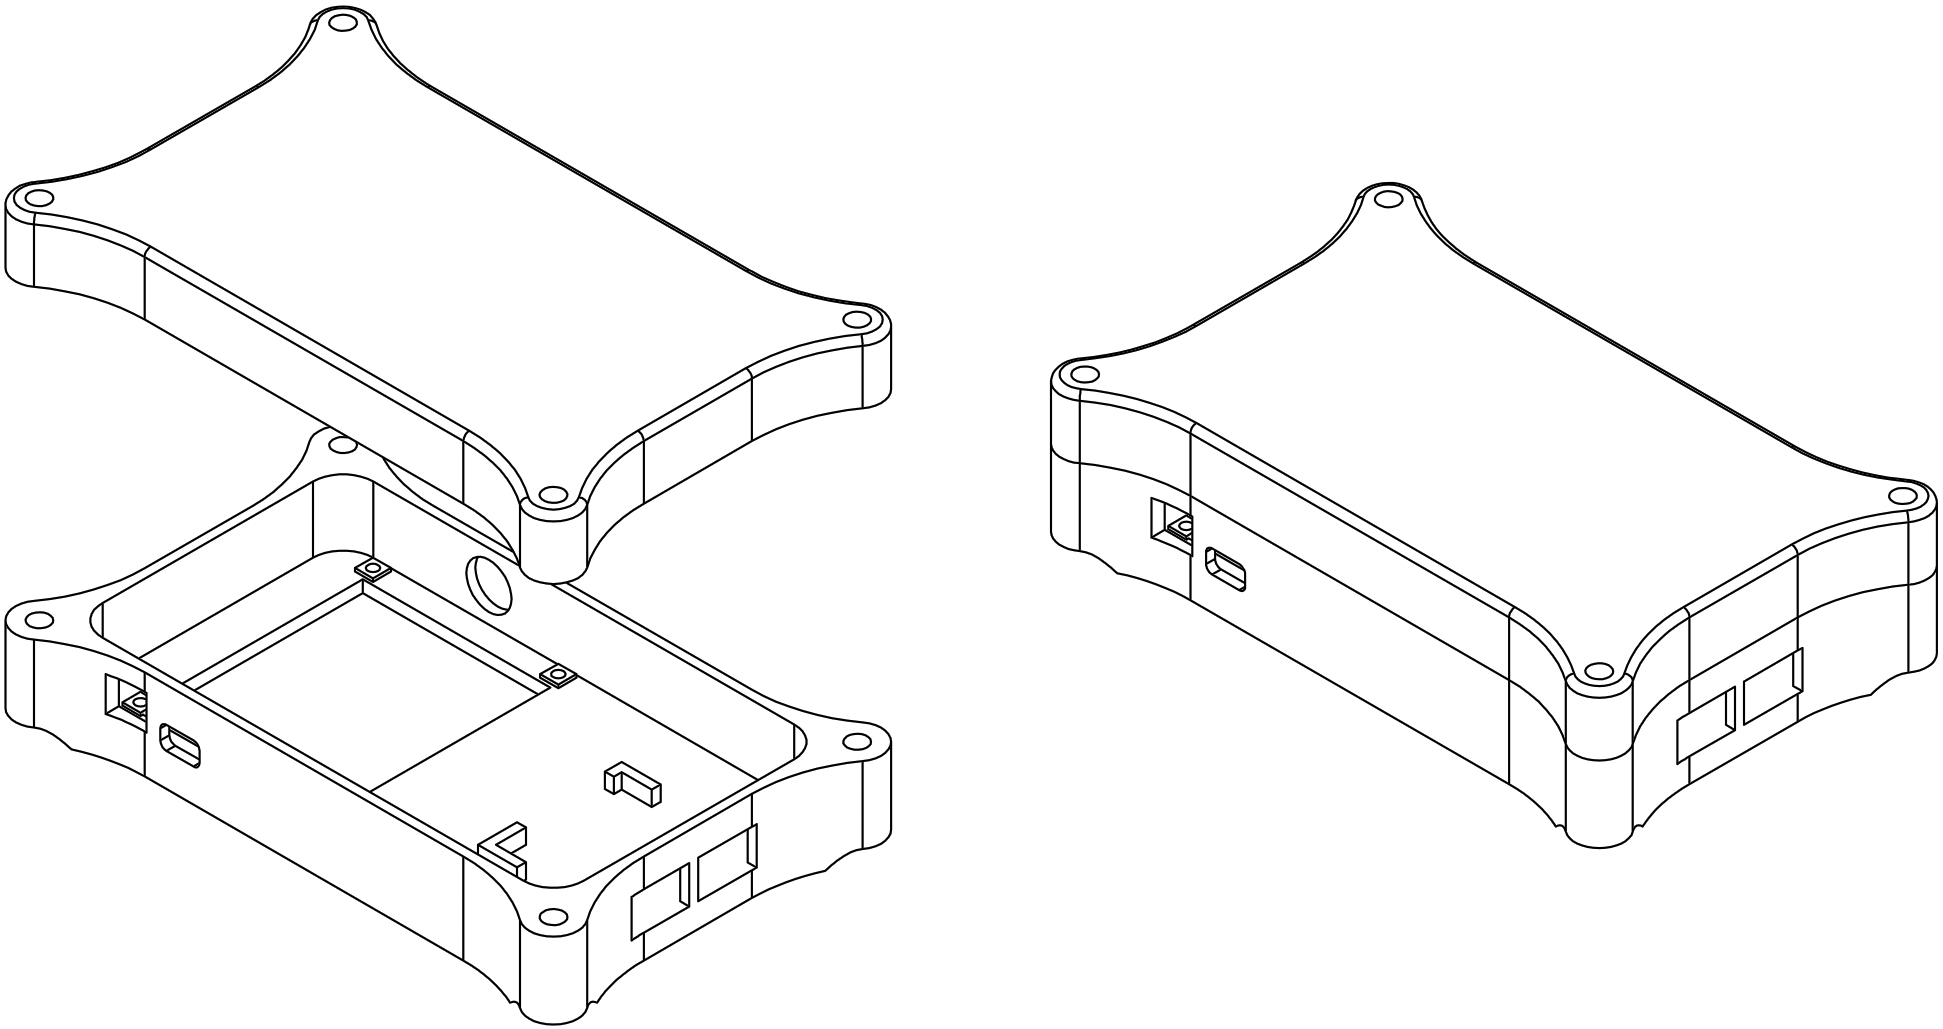
\includegraphics[width=3.5in]{img/enclosure_1.png}
    \caption{An exploded, isometric view of the enclosure.}
    \label{fig:enclosure-exploded}
\end{figure}


In order to place the other system components in an ideal location for gathering data, a physical enclosure was needed. The enclosure was designed with the goal of being able to be mounted on a vertical wall or other flat surface. The enclosure houses all of the previously described system components, including the PCB, the SPS30, and the battery. Holes were included for the USB-C connector, solar panel connector, and antenna. Additionally, specific intake and outtake holes were created for the SPS30, in accordance with the guidelines specified in the datasheet \cite{sps30-datahsheet}. Two extrusions were made on the bottom part of the enclosure to keep the SPS30 from sliding horizontally within the enclosure. A third extrusion was made coming down from the cover to keep the SPS30 from moving vertically. 

The design includes four holes on each corner for inserting screws, in order to lock the cover in place. The full enclosure design can be seen in Figure \ref{fig:enclosure-exploded}. The enclosure was 3D printed using black PLA+ as the material. This specific type of PLA has additives that are designed to improve the material's rigidity.

\section{System Design}
The Aether Node is responsible for periodically reading sensor measurements from the three sensors and transmitting them over \lorawan to be stored and displayed on a web user interface. This is done by integrating all of the previously discussed components into a single, cohesive design. This design can be broken down into three major parts. The first is the power subsystem; this part is responsible for handling the power input from the battery and solar panel and converting into a usable form for the other parts of the system. The second part is the USB power and data; this part is responsible for allowing the system to charge and communicate over USB. The third and final part is the circuit integrating the sensors with the microcontroller; this part is responsible for getting data from the sensors to the microcontroller.

\subsection{Solar Panel and Charging Subsystem Design}
The Aether Node is powered by a Li-ion battery and is designed to operate entirely off-grid. It is equipped with the ability to charge the Li-ion battery through a 6 V solar panel or through a USB-C cable. This provides the user the flexibility to directly charge a depleted battery and keep the system operational in situations where the solar panel cannot provide sufficient power. Such issues could be a result of poor weather or a damaged solar panel. 

Charging the system with a solar panel means a filtering capacitor will be needed to stabilize the solar panel. A relatively large 4700 mF capacitor will be used for this design. Additionally, a diode is included to ensure that no voltage is leaked out by the capacitor. A schematic showing the solar panel circuit can be seen in Figure \ref{fig:Solar_Panel}. This power subsystem of this design also incorporates smart load sharing, meaning that the power inputs can efficiently charge the Li-ion battery, while also powering the system. The battery is only used when either the solar panel cannot meet system load requirements or both the solar panel and USB inputs are not present.

\begin{figure}[b]
    \centering
    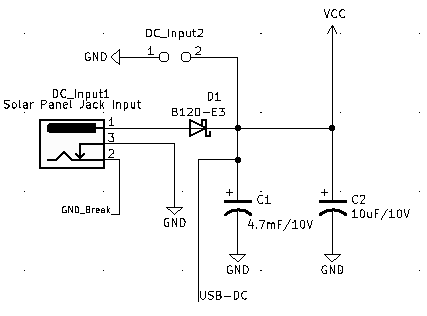
\includegraphics[width=3.5in]{img/Solar_Panel.PNG}
    \caption{The schematic for the solar panel circuit.}
    \label{fig:Solar_Panel}
\end{figure}


The MCP73871 battery charge management controller will be responsible for a voltage proportional charge control feature that will optimize the solar cell and will also allow the USB input to power the system. This feature is used to maximize solar performance, as opposed to using maximum power point tracking (MPPT) tracking. This is because, for low voltage applications, such as this design, MPPT is not that much more efficient than a linear charge controller and would only increase size and cost of the design if implemented in this design. 

In order to keep costs to a minimum, it was decided that the low increase in efficiency was not worth the increase in cost. A maximum charge rate of 500 mA is outputted by the charge controller and it is adjustable from 50 mA to up to a 1000 mA charge rate. The system is designed to draw the maximum amount of current possible, depending on the set maximum charge rate, from the solar panel to meet load requirements. If the load requires more current, or the solar panel reaches a certain low-voltage threshold, the system will then turn to the battery to meet the system load requirements. This smart load sharing automatically uses input power if available, which prevents the battery from frequently charging and discharging and thus extending the battery life. 

Three status LEDs are used to indicate the charging status of the battery, which are as follows:

\begin{enumerate}
\item Power on
\item Charging in progress
\item Charge done
\end{enumerate}

At the output end of the charge controller will be a linear dropout regulator (LDO) used to drop down the voltage to a constant 3.3 V, which will be used as the main power rail for the system. Additionally, a thermistor connected to the charge controller is used to constantly measure the temperature of the Li-ion battery to ensure the battery is not charged in unsafe temperature conditions. This charge controller circuit can be seen in Figure \ref{fig:charge_controller}.

\begin{figure}
    \centering
    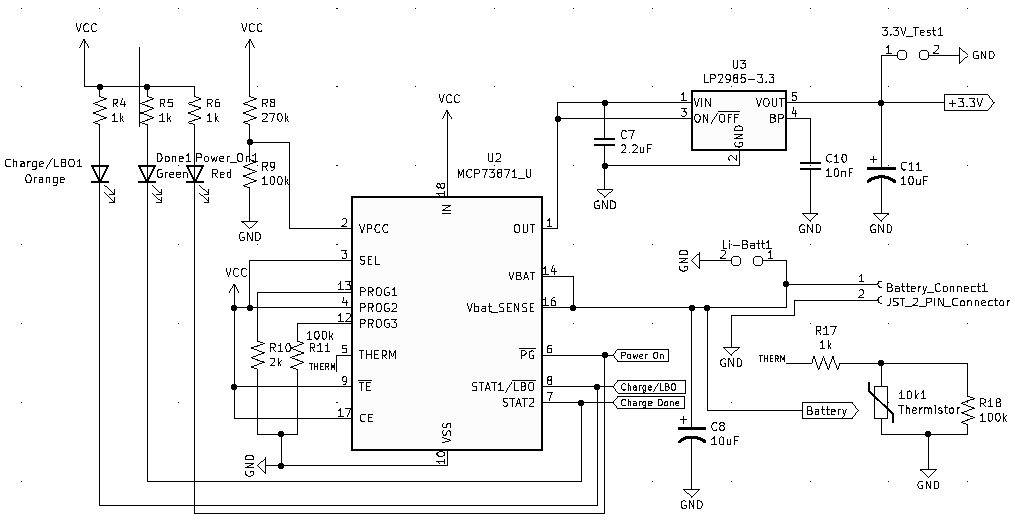
\includegraphics[scale=0.65,angle=270,origin=c]{img/Charge Controller.PNG}
    \caption{The schematic for the charge controller circuit.}
    \label{fig:charge_controller}
\end{figure}

\subsection{USB Power and Data}
This design incorporates a USB-C port that charges the system in the cases where either a solar panel is not used or the solar panel cannot meet the required system load. Additionally, a USB-to-UART circuit is implemented in the design to translate USB communication data to a UART interface. This is essential because host communication will be done through USB input. Since the LoRa-E5 can only interface over UART, a conversion IC is required. This design uses the Silicon Labs USBXpress Family CP2102N chip to achieve this. 

The USB power design also includes ESD diode circuit protection to clamp any high voltage peaks and prevent system damage in the case of an electrostatic discharge event. The Data(D-) and Data(D+) pins on the bridge are connected to the same pins on the USB and are separated by the protection circuit previously discussed. The TX and RX pins are connected to the USB serial RX and TX pins on the microcontroller. LED diodes are set in place to indicate that a proper communication link has been established. The circuit schematic for the USB-to-UART interface showing the ESD diode protection circuit can be seen in Figure \ref{fig:USB_UART}. 

\begin{figure}
    \centering
    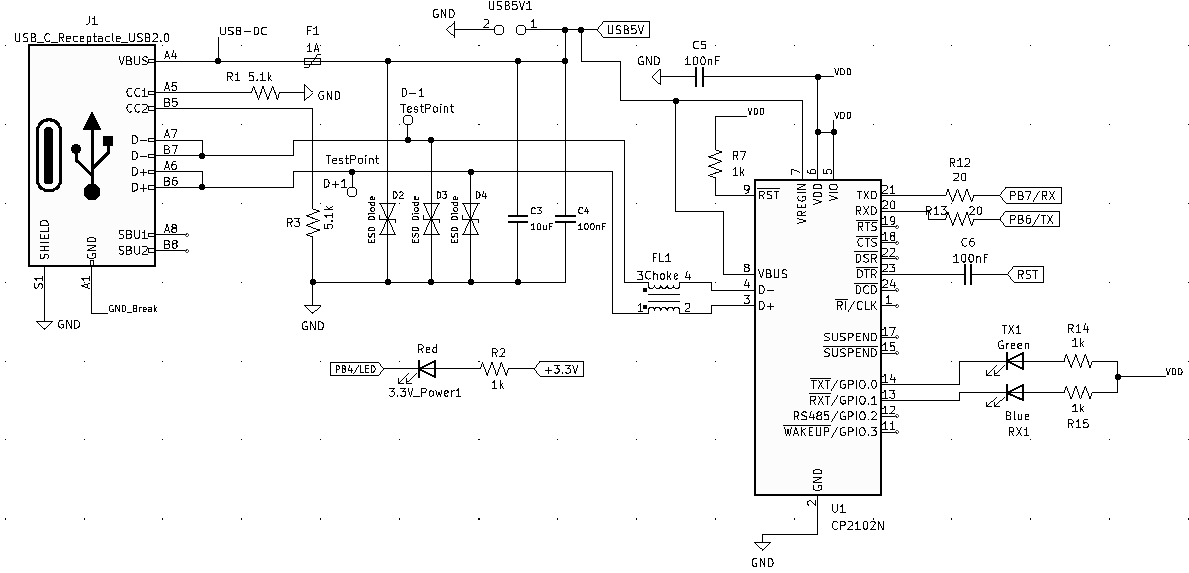
\includegraphics[scale=0.75,angle=270,origin=c]{img/USB_UART.PNG}
    \caption{The schematic for the USB-to-UART circuit.}
    \label{fig:USB_UART}
\end{figure}

\subsection{Sensor Circuits}
The three main sensors in this circuit are connected to the LoRa-E5 microcontroller via each sensor's respective Serial Clock(SCL) and Serial Data(SDA) pins. \iic is used as the communication interface for all sensors. If a sensor has more than one communication interfaces available, the appropriate circuit configurations are used to ensure that \iic is used.

\subsubsection{BME688 Sensor}
 To use the \iic interface on the BME688, the VDDIO on pin 6 is connected the chip select status (CSB) on pin 2. To power the sensor, VDD on pin 8 is connected to the 3.3 V power rail and to VDDIO. Both VDD and VDDIO are paired with decoupling capacitors that are connected to ground to help oppose fast changes of voltage. The pins dedicated to the I2C communication interface are serial clock (SCL), data (SDA), and slave address LSB (SDO). Because SDI is bi-directional, it is connected to VDDIO via a pull-up resistor. 
 
 Once the \iic interface is connected, the next step is to make the appropriate connections to the LoRa microcontroller. The serial data input (SDI) on pin 3 is directly connected to the serial data (SDA) on pin 6 on the microcontroller. The serial clock (SCL) pin on the BME688 is connected to pin 5 on the microcontroller. The SDO pin on the BME688 is tied to ground for the default slave address.
 
\subsubsection{ZMOD4510 Sensor}
The serial clock and serial data pins for the \iic interface on the sensor module will be connected to the respective pins on the microcontroller, which are pins 5 and 6. VDD is the voltage supply for the ZMOD4510 itself and VDDH is the voltage supply for the integrated heater inside the ZMOD4510. The VDDIO pin is the voltage supply for I/O interface in the ZMOD4510. These three voltage supply pins will all be connected to the 3.3 V power rail. 

Pin 3 on the ZMOD4510 is the interrupt pin on the sensor. This pin will read HIGH when a measurement is running and LOW when a measurement has finished. It will be connected to GPIO pin 11 on the microcontroller. The ZMOD4510 is equipped with a RES function on pin 11. This is an active low pin, which is connected to the 3.3 V power rail via a 10 \kOhm pull-up resistor.

\subsubsection{SPS30 Sensor}
 To us the \iic interface on the SPS30 sensor, the select (SEL) pin must be tied directly to ground. This particulate matter sensor operates with a 5 V input, which is the reason that a 5V power rail was added to the design of the Aether Node through the use of a DC-to-DC boost converter. The Li-ion battery was used to power the boost converter that will output the required 5 V for the SPS30. This boost converter circuit can be seen in Figure \ref{fig:5V}. The VDD pin on the SPS30 is the supply voltage pin that will be powered by this 5 V rail. A 3.3 V input was used instead of 5 V for the SDA and SCL pins, because the pins are Low Voltage Transistor to Transistor Logic (LVTTL) 3.3 V compatible. Using 3.3 V instead of 5 V for the \iic pins ensures no over-voltage damage is done to the microcontroller since it operates under the 5 V range.
 
 \begin{figure}
    \centering
    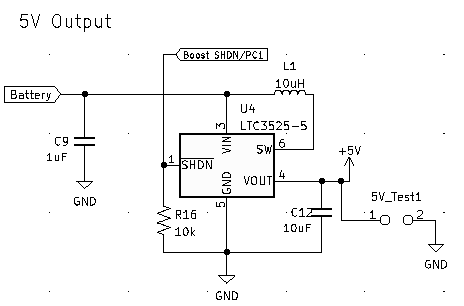
\includegraphics[[width=3.5in]{img/5V.PNG}
    \caption{The schematic for 5V boost converter circuit.}
    \label{fig:5V}
\end{figure}

\subsection{Microcontroller}  The chip is powered through VCC on Pin 1 which takes 3.3 V from the main power rail. The serial clock and serial data pins for \iic are located on pins PB15 and PA15 respectively. These are the pins used to communciate with the system sensors. The respective pins on each sensor will be connected to PB15 and PA15 so sensor data can be read at defined intervals. Pin 15 is the RFIO pin which will be connected to the antenna. Additionally, 3 GPIO pins were used to read the 3 status states of the battery charge controller.

\section{System Firmware}
The firmware running on the Aether Node is written in C and is using Zephyr, an open-source, real-time operating system being maintained by Nordic Semiconductor. \footnote{The Zephyr website: \texttt{https://www.zephyrproject.org/}} One of the major distinguishing features of Zephyr, which is one of the primary reasons as to why we used Zephyr over more more popular RTOSes, such as FreeRTOS, is its use of a consistent device driver model. Zephyr provides a consistent device model for configuring the drivers that are part of the platform and a consistent model for initializing all the drivers. This makes drivers more straight forward to implement. Additionally, devices become much easier to interact with in the application code. For example, in Figure \ref{fig:dev_bme}, we demonstrate how to initialize a device and take a reading from a sensor. Many details, such as the \iic address of the device, are abstracted away when using Zephyr.

\begin{figure}
\begin{Verbatim}[frame=single, language=C, fontsize=\footnotesize]
const struct device *dev_bme;
dev_bme = DEVICE_DT_GET(DT_NODELABEL(bme688));
sensor_sample_fetch(dev_bme);
sensor_channel_get(dev_bme, 
                   SENSOR_CHAN_AMBIENT_TEMP, 
                   &temp);
\end{Verbatim}
\caption{An example of initializng the BME688 and getting a temperature reading using the Zephyr device model.}
\label{fig:dev_bme}
\end{figure}

The design of the firmware is best thought of in terms of three separate control loops. Those controls are the sensor control loop, the LoRa control loop, and the serial command control loop. Additionally, there is a power management component that is implemented in the firmware. This power management involves putting the LoRa-E5 in a low-power state when the system is idling and cutting the power to the SPS30 when it is not taking readings. 

\subsection{Sensor Control Loop}
The sensor control loop is responsible for collecting data from the three sensors used by the system (BME688, ZMOD4510, and SPS30). A thread is dedicated to each sensor for the execution of this control loop. Due to the fact that each sensor follows the same control flow, Figure \ref{fig:firmware} depicts each sensor thread running the same tasks in parallel. 

The following description of the sensor loop follows the sample code seen in Figure \ref{fig:sensor_loop}. When the thread is started by the kernel, it begins by initializing the sensor. Next, the sensor takes a reading. In Zephyr, this is done by first calling \texttt{sensor\_sample\_fetch(dev)}, which calls the appropriate driver function to take a sensor reading. The results from that function are then stored in a sensor channel variable. To access that value, a call to \texttt{sensor\_channel\_get()} is made. After accessing all of the sensor readings for that sensor, the results are converted to the CayenneLPP\footnote{This is a simple data packet structure designed for storing sensor data. It follows the format: 1 byte for sensor type, 1 byte for data type, and then $n$ bytes for the data payload \cite{cayenne}.} format and placed in the message queue, where the data will later be read by the LoRa thread. Finally, the thread is put back to sleep by calling \texttt{k\_msleep(DELAY)}. In the case of our final design, this delay was set fifteen minutes. This also allows the kernel to schedule other threads to run. 

\begin{figure}
\begin{Verbatim}[frame=single, language=C, fontsize=\footnotesize]
const struct device *dev_bme;
dev_bme = DEVICE_DT_GET(DT_NODELABEL(bme688));

while(1) {
    sensor_sample_fetch(dev_bme);
    sensor_channel_get(dev_bme, 
                   SENSOR_CHAN_AMBIENT_TEMP, 
                   &temp);
                   
    k_msleep(DELAY_15_MINUTES);
}
\end{Verbatim}
\caption{A code snippet that shows the basic structure of the sensor reading loop. This example is for the BME688 and only shows getting a temperature reading.}
\label{fig:sensor_loop}
\end{figure}

% How many times will it attempt to send?
\subsection{LoRa Control Loop}
This is the control loop that handles sending collected sensor readings to our server over LoRaWAN. It begins by first checking if there are any messages containing sensor data in the message queue. If the message queue is empty, the thread yields until notified by another thread when a message is inserted into the queue. If there is a message, it removes it from the queue, and as many messages that can fit within the LoRaWAN packet as defined by the current data-rate, and then attempts to send the LoRaWAN message. The loop then waits for the message to send successfully. If it does not send successfully the first time, the thread will attempt to send the message up to 10 times.

\subsection{Serial Command Control Loop}
This is the control loop that handles accepting user commands from the UART shell. As shown in Figure \ref{fig:firmware}, the design design was able to use Zephyr's built-in shell API. Adding the shell to the firmware only involved adding a few options to the project configuration file. Regarding the functionality of reading data from connected sensors, the default Zephyr shell already included the ability to read sensors connected to the \iic bus. %A new shell command was added using the shell API to configure the LoRaWAN parameters of the Aether Node.

\begin{figure}
    \centering
    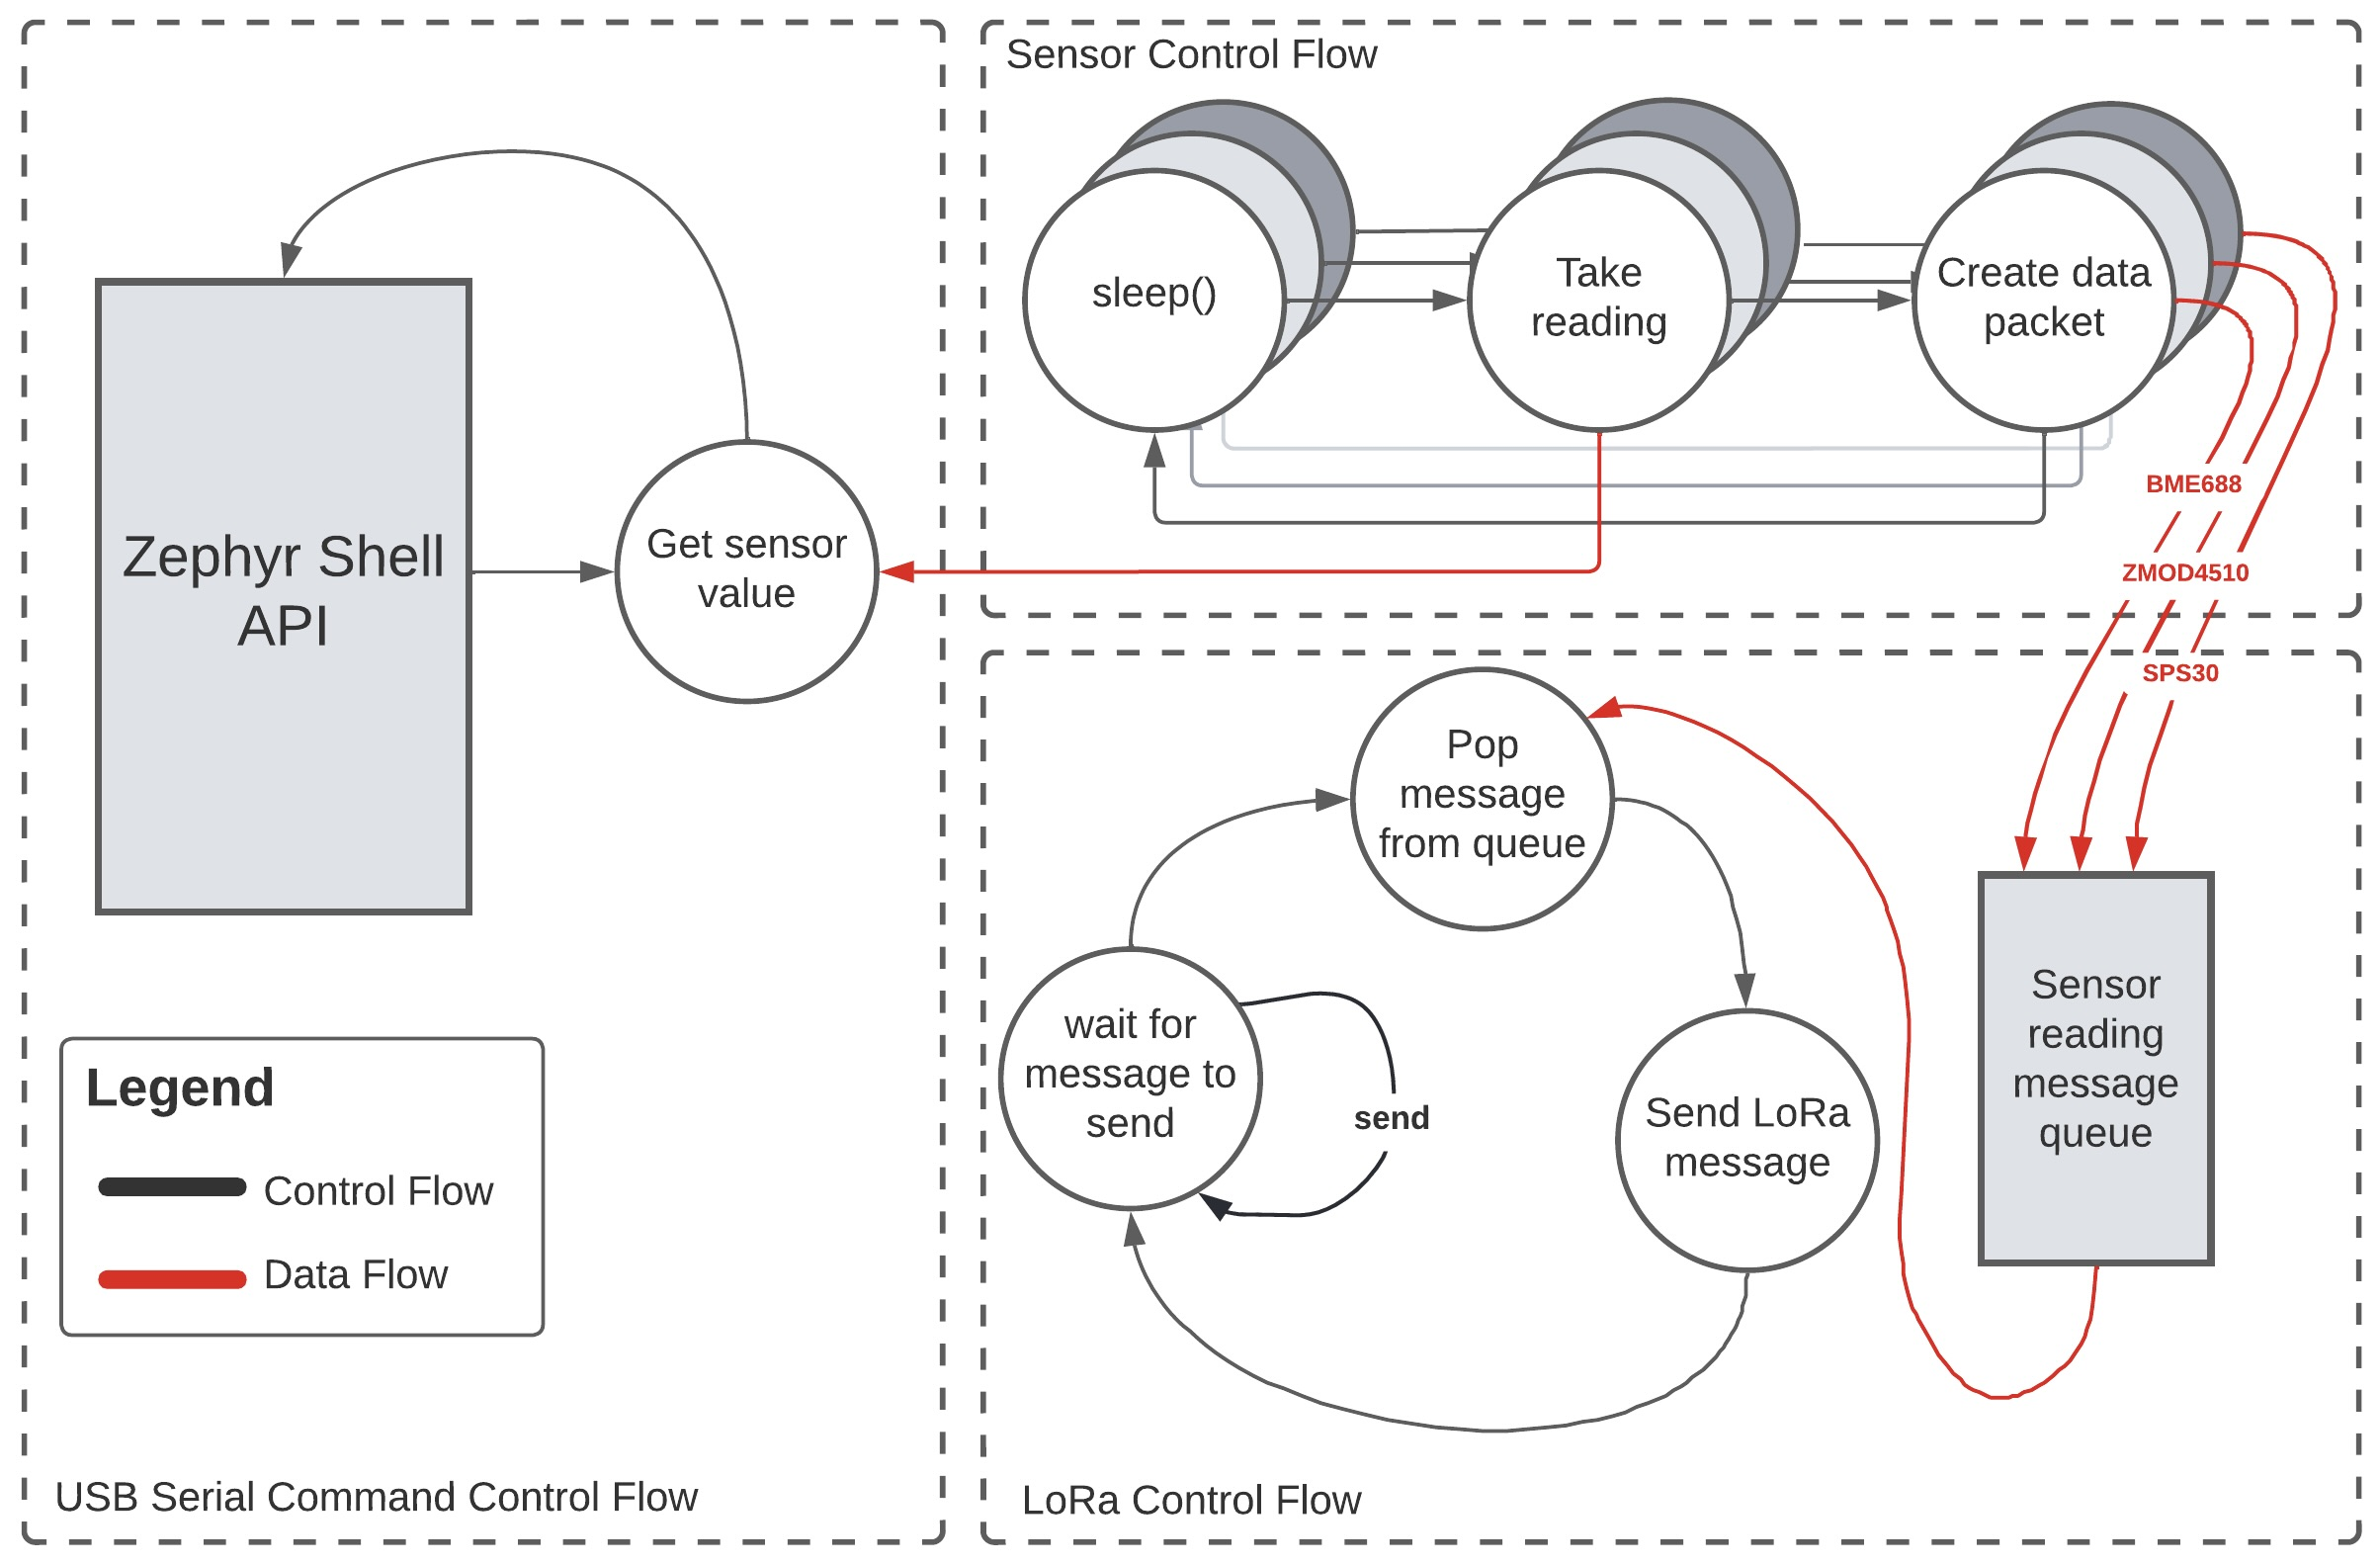
\includegraphics[width=3.5in]{img/firmware_diagram.jpeg}
    \caption{A state diagram showing the general flow of our device firmware.}
    \label{fig:firmware}
\end{figure}

\subsection{Power Management}
Power management was necessary to allow the Aether Node to operate for a longer period of time. The two primary power management features implemented in the firmware was power-gating the SPS30 and putting the LoRa-E5 in a sleep mode when not taking sensor measurements.

The power-gating of the SPS30 was implemented by using the Zephyr power domain API. The power domain toggles a GPIO pin on the MCU that toggles the power to the SPS30. Before calling the sleep function in the SPS30 thread, a function is called to turn the power domain off. Similarly, before calling \texttt{sample\_fetch(dev)}, the power domain is turned on.

The LoRa-E5 was put into a sleep mode when not taking sensor measurements. This was implemented using the Zephyr power management API. This involved setting up multiple power states by defining them in the Devicetree file. We defined both \texttt{enable\_sleep()} and \texttt{disable\_sleep()} functions using the appropriate API calls. This allowed us to call \texttt{disable\_sleep()} before starting to sensor reading and then call \texttt{enable\_sleep()} before putting the sensor thread back to sleep.


\section{Website and User Interface}
A web application was chosen to be used as the primary user interface. This decision was made due to the fact that the internet is widely available and we wanted the sensor data to be easily accessible. As shown in \ref{fig:overall-bd}, device packets are transmitted over \lorawan to our gateway running The Things Stack software, which forwards the packets to the Things Stack online service. These packets are sent to our backend, running on Supabase, and the data is displayed on our web client.

\subsection{API and Database}
Upon being processed in The Things Stack, the packets are sent as event messages to our backend, through REST POST requests. Our backend, runs almost entirely on Supabase, a managed and pre-configured PostgreSQL database. Supabase comes pre-enabled with PostgREST, an extension for PostgreSQL, that allows the database to be accessible through REST. We then use the Supabase JavaScript client for the web application front-end to access the data and setup real-time subscriptions to updates in the database, using Supabase's "real-time" service. The real-time service uses the replica-set features of Postgres, and must be enabled on a table-by-table basis. For our application, we receive updates for the \texttt{reading}, \texttt{hourly\_reading\_stats}, and \texttt{raw\_hourly\_aqi} tables and display the updates on the map and real-time graphs.

As for handling \lorawan uplinks, we have a database function called \texttt{handle\_lorawan\_uplink} that is exposed through a REST remote procedure call endpoint \texttt{/rest/v1/rpc/handle\_lorawan\_uplink}. The uplink handler reads the The Things Stack uplink event JSON file and decodes the Cayenne-formatted, base64-encoded payload using another database function, but this time written in JavaScript using another Postgres extension. Postgres has extensive support for JSON and JSONB (binary JSON) data types and makes it easy to work with, since there are special operators and functions for manipulating JSON blobs. The data-flow for this can be seen in Figure \ref{fig:dataflow}.

Once decoded, all sensor samplings are inserted into the \texttt{reading} table in the database. Triggers are setup to check for alerts, update device and user metadata, and update the hourly values for each sensor channel in a table called \texttt{hourly\_reading\_stats}. Finally, once the hourly statistics are updated, a trigger updates the hourly raw AQI. The raw AQI is the AQI directly calculated from the hourly reading statistics, and does not perform any linear regressions. There is also a trigger on the \texttt{raw\_hourly\_aqi} table to check for alerts on the different types of AQI. If we had more time, we would have liked to implement the EPA NowCast, which uses the partial lease squares linear regression. Alerts are sent as POST requests to a transactional email service, MailerSend. MailerSend is configured to send emails from our domain. The data-flow for this can be seen in Figure \ref{fig:dataflow}.

\begin{figure}
    \centering
    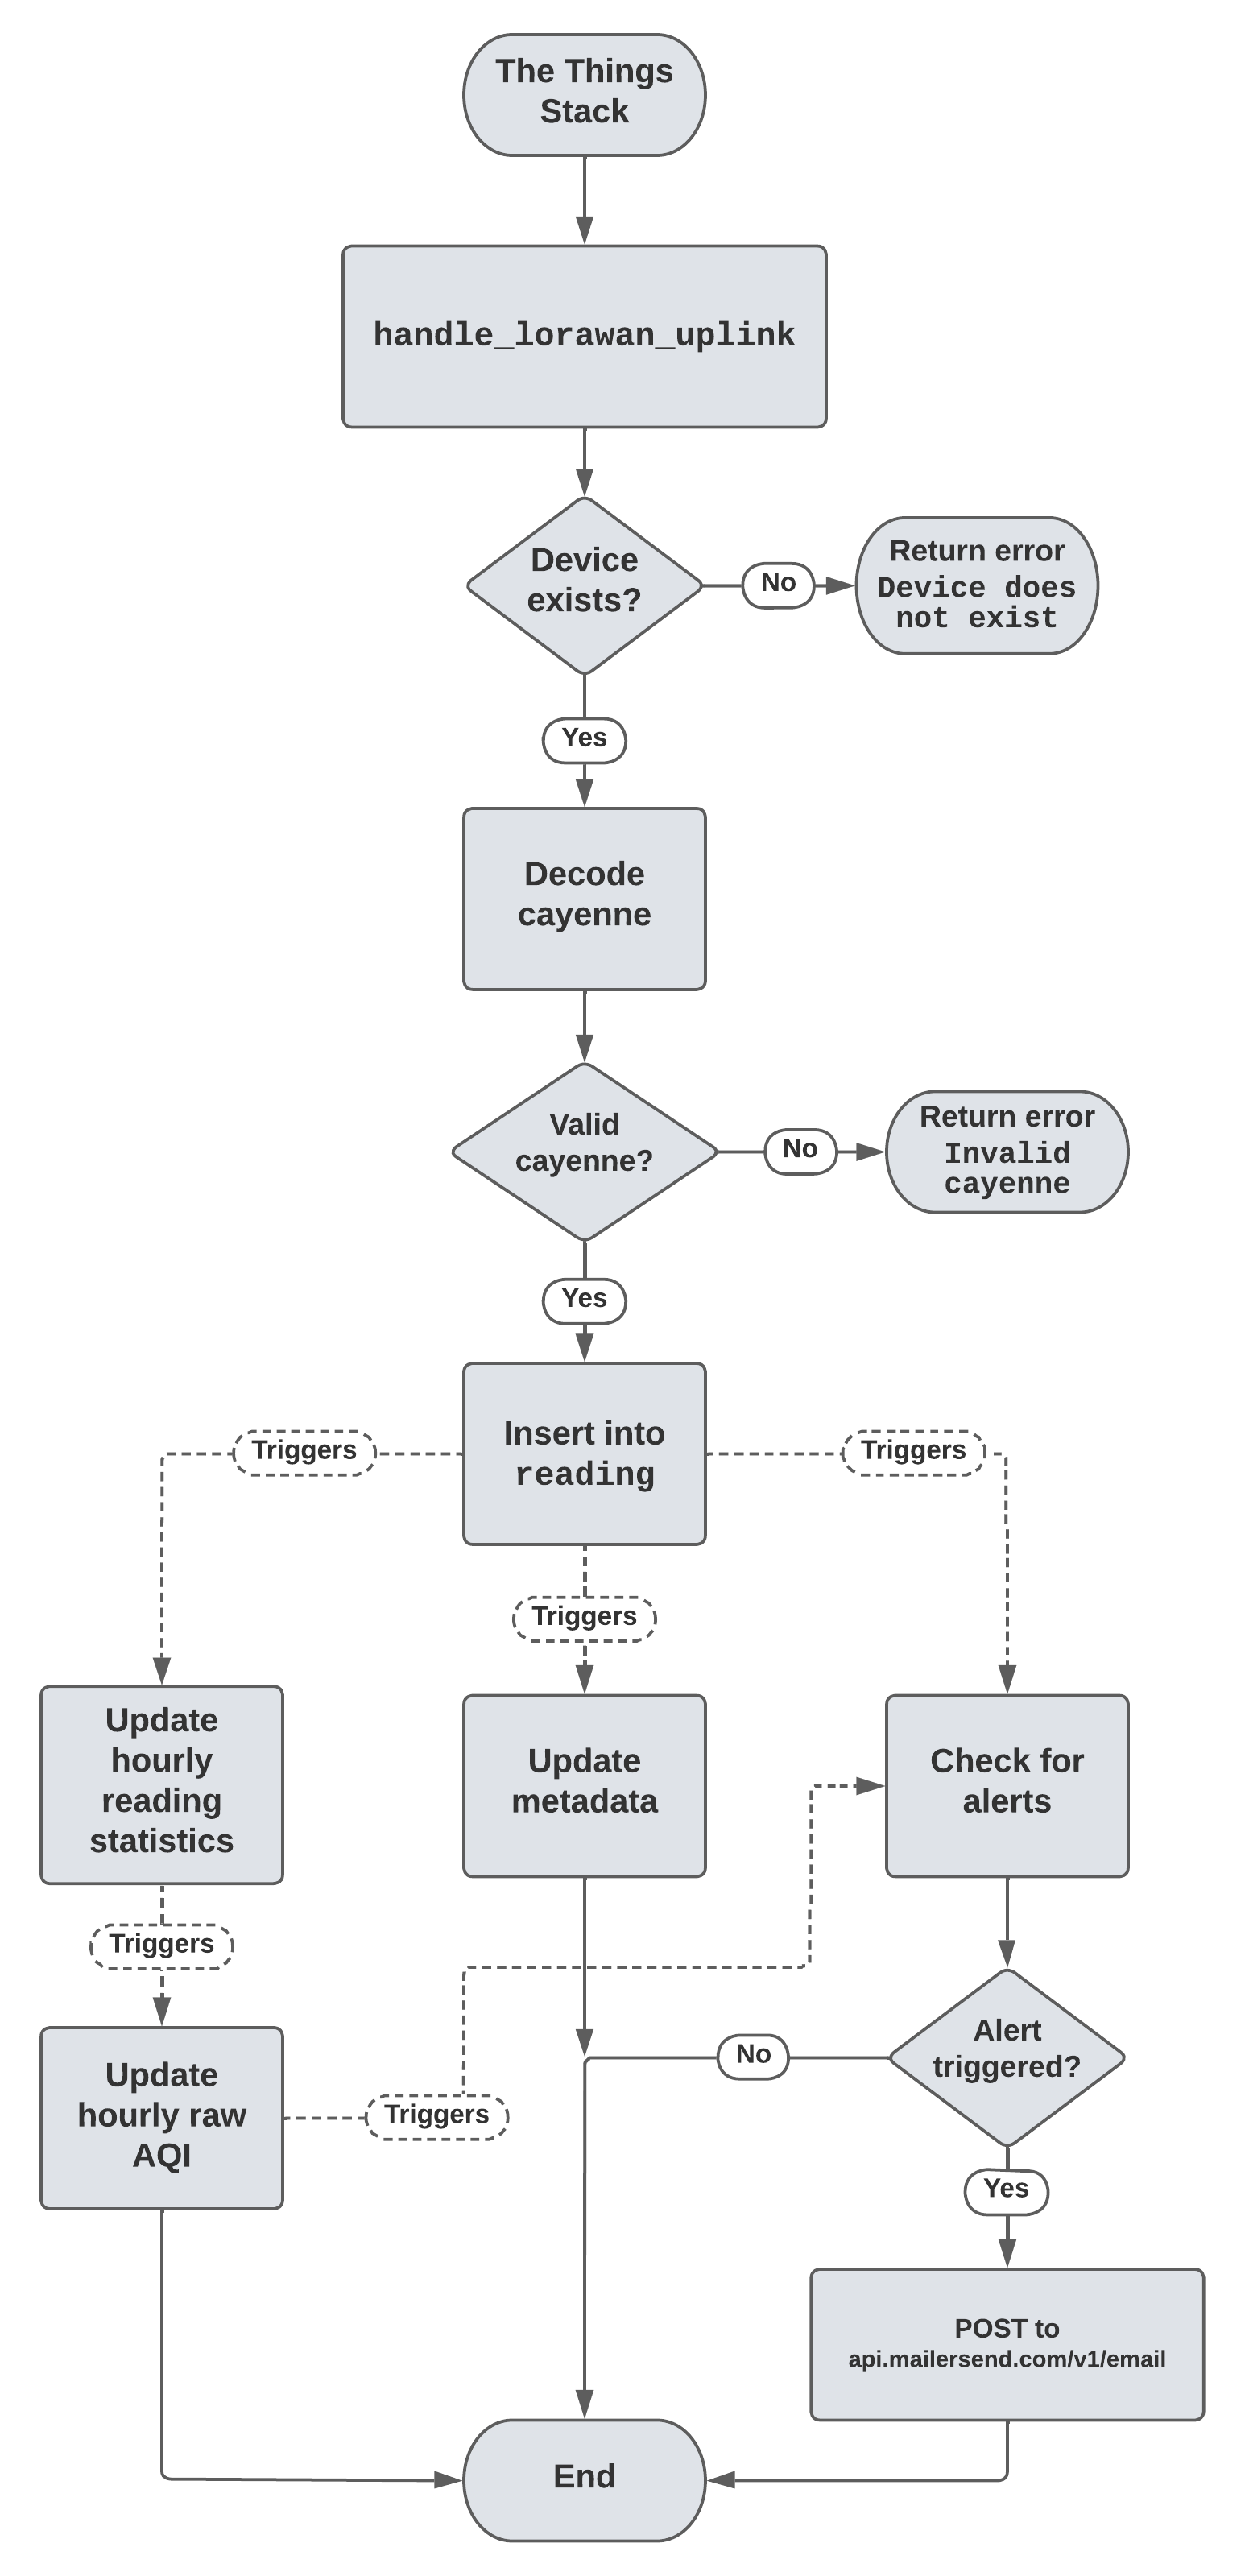
\includegraphics[scale=0.45]{img/db-dataflow.png}
    \caption{The general data-flow for data originating from The Things Stack to where it is stored in Supabase.}
    \label{fig:dataflow}
\end{figure}

\subsection{Web Application}
The web application\footnote{The Aether website can be be accessed at the following address: \texttt{https://aethersensor.network}} is where anyone can view the air quality in their local area, given that there is an Aether Node nearby. The web application shows a map and sidebar on the homepage, as shown in Figure \ref{fig:website}. Each type of data to be displayed on the map, is known as a "layer". There are layers for the different types of AQI (O$_3$ and O$_3$ + PM), PM, O$_3$, temperature, relative humidity, and air pressure. For each layer, there is a unique legend that maps the colors of the data on the map to a numerical value. If a user does not have an account, they can view data, but they cannot see device or user specific information. Users with an account can see and modify their own devices. Devices can be viewed on the map by enabled the "Show" toggle in the sidebar. Users can see device metadata and view real-time and historical values by clicking on their device name in the sidebar.


\begin{figure}
    \centering
    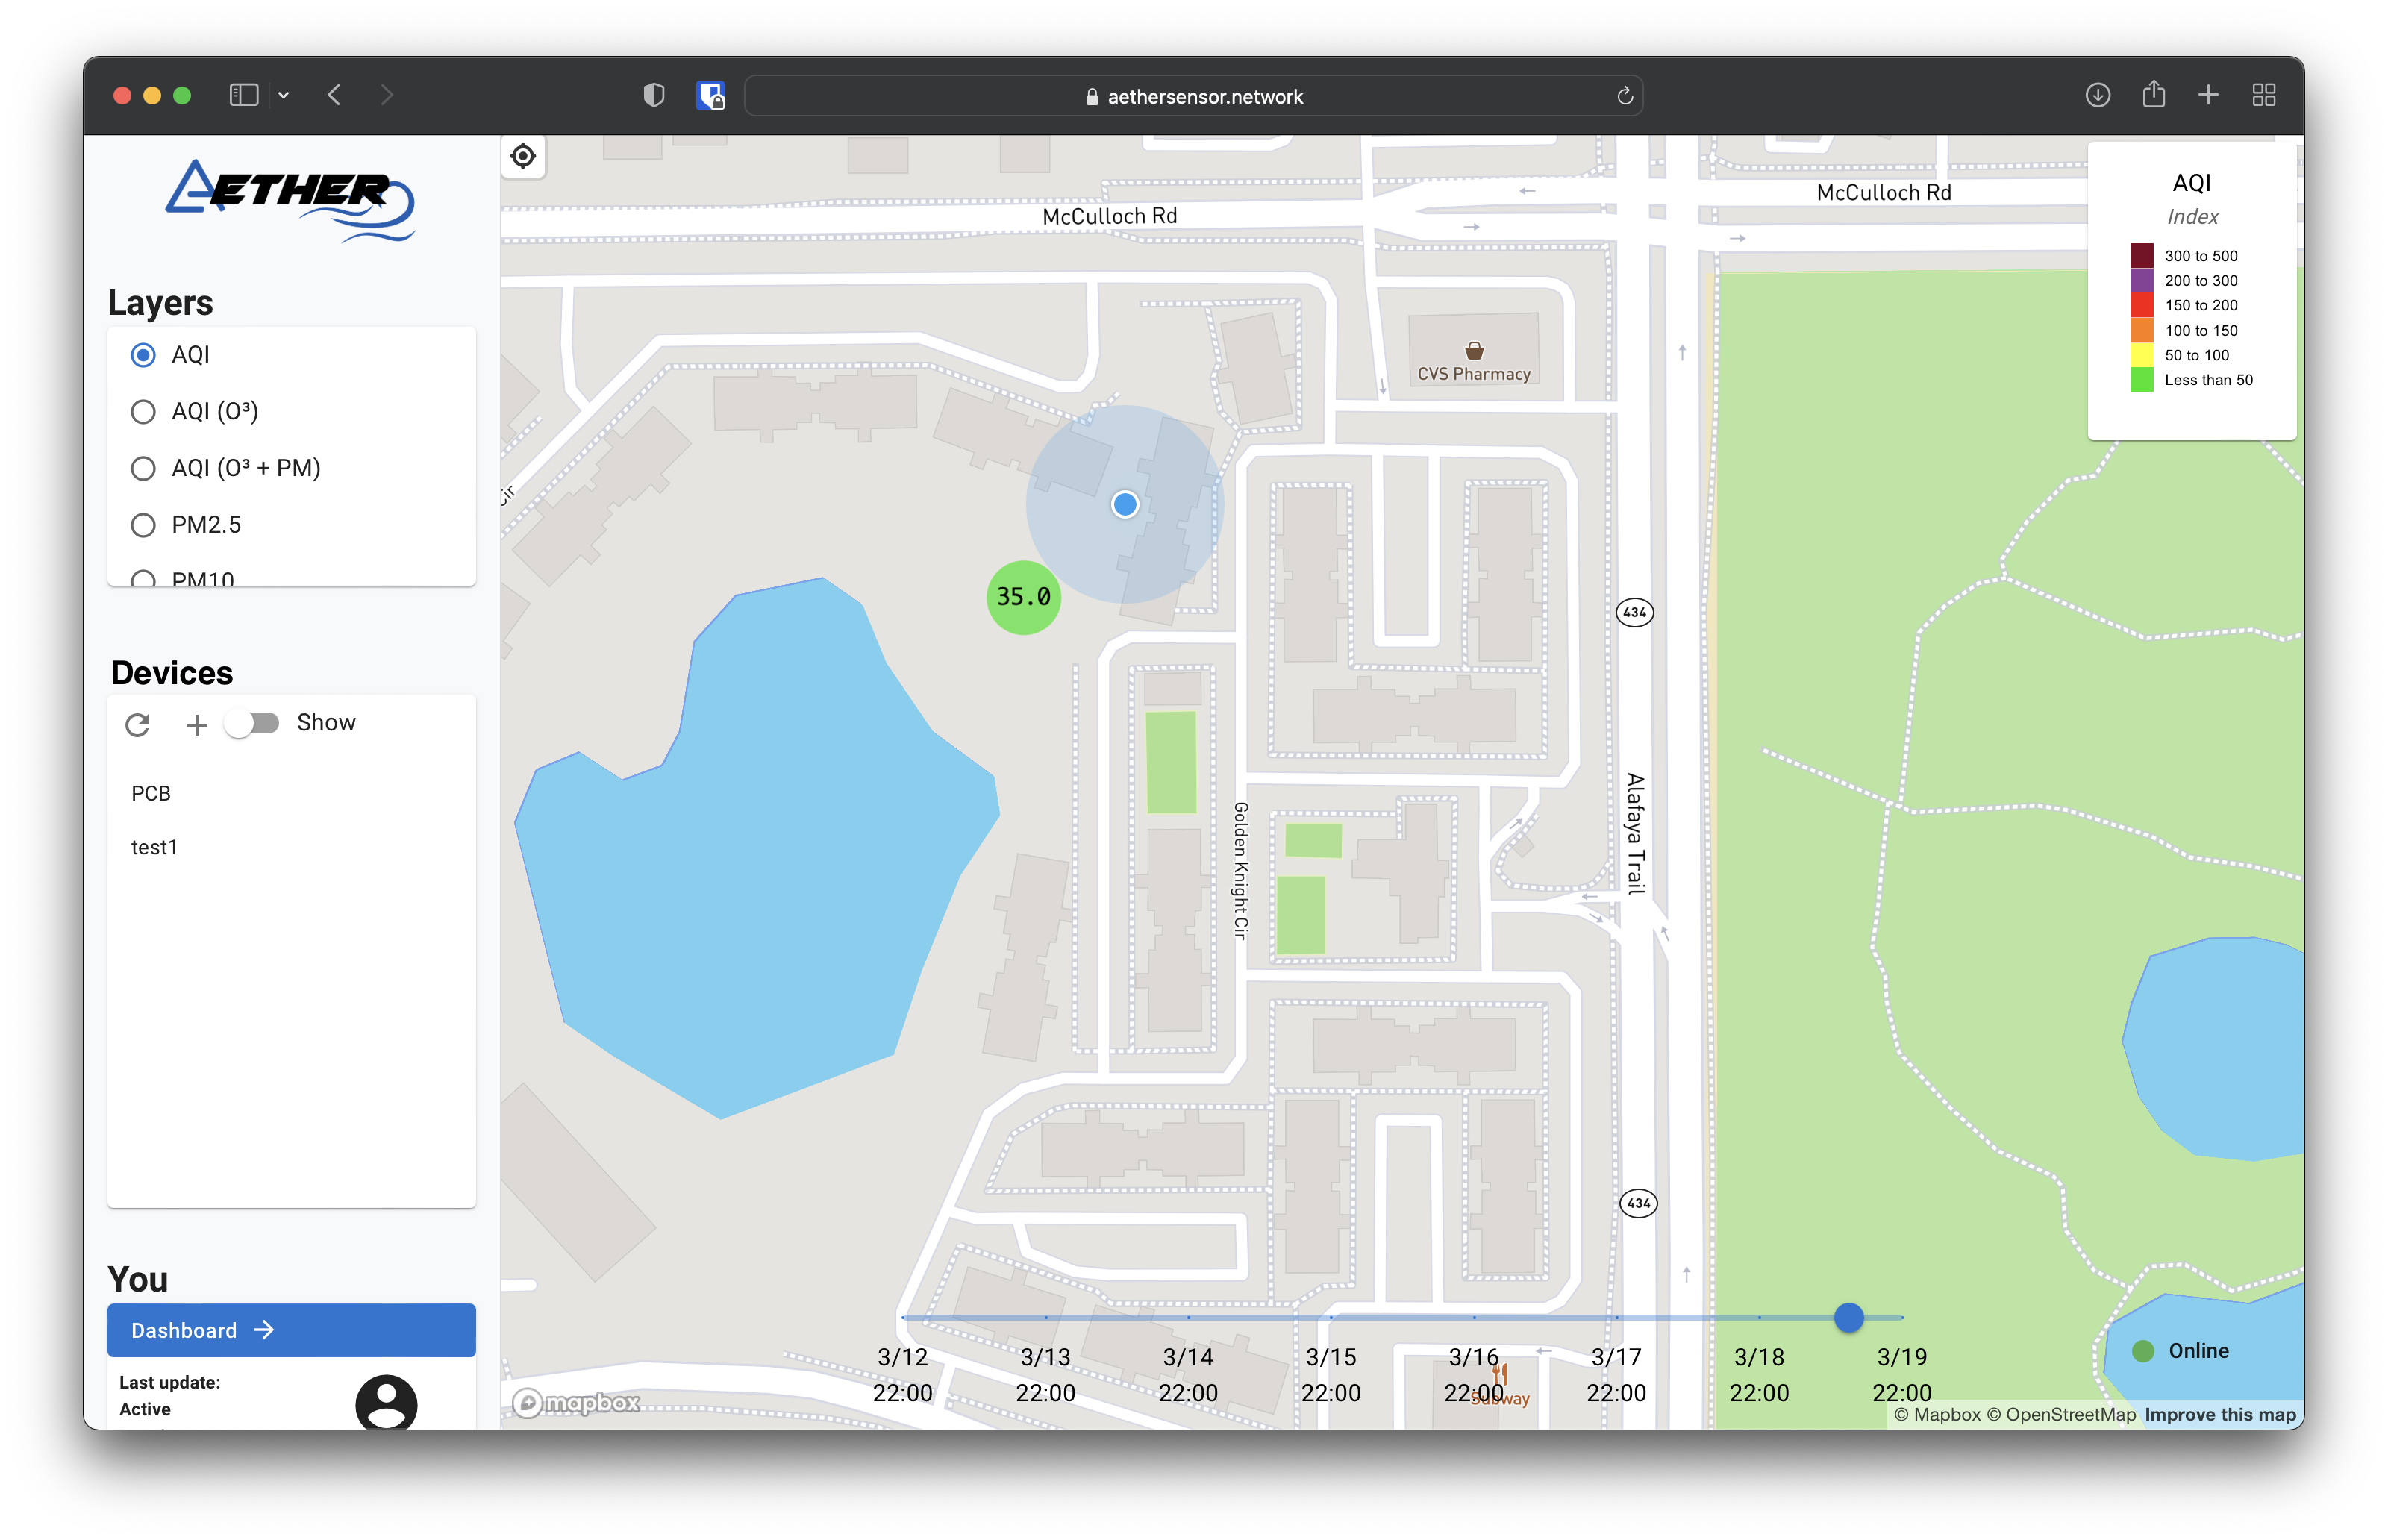
\includegraphics[width=3.5in]{img/website.png}
    \caption{An image of the Aether website showing an AQI reading overlaid on a map.}
    \label{fig:website}
\end{figure}


\section{Conclusion}
This two-semester project has been a valuable experience to grow both our team's technical knowledge as well as our ability to effectively function as members of larger project. The end result of our multiple months of effort was a fully-functioning prototype that met our requirements. Our team was able to successfully build both Aether Node, which included a custom PCB and enclosure, as well as the Aether website, which allowed users to view the data collected by the Aether Node.
% The result of the project was a successful construction of the Aether node network with a functioning prototype gateway and node. Both the physical device used to collect data, as well as the web server used to receive and display that data were built and met all the design constraints we put in place. The four layer PCB was design from scratch, assembled and housed in a 3D printed enclosure. On the PCB is a Seed LoRa-E5 LoRaWAN module used to connect our devices just like many new technologies utilizing the growing in popularity Internet of Things(IoT). This module packages a ST STM32WLEIC, an Soc using both an ARM M4 processor and a LoRa chip. The LoRa chip receives data from our gas sensors the BME688, the ZMOD4510, and the SPS-30. These sensors give us a read out for several gases in the air, humidity, temperature, and even particulate matter. These readouts can then be transmitted to the database hosted on Amazon Web Services(AWS) and the results will be configured on a web page utilizing a javascript framework. The final product is a web application that will give users an overview of air quality overlaid on an OpenStreetMaps map. At the end of this project our team has taken pride in the fact that we have created something that can be used for the common good and we are thankful to UCF for giving us all the tools and capabilities to make this project happen.

\section*{Acknowledgment}
We have a couple that we would like to acknowledge for providing us assistance or contributing to our project in some way. To start, we would like to acknowledge Dr. Samuel Ritchie. Dr. Ritchie provided us with guidance on how to approach meeting the requirements for Senior Design. We would also like to acknowledge Dr. Lei Wei. Dr. Wei provided us with invaluable feedback numerous times throughout the design process. Finally, we would like to thank Porter Morgan. Porter gave us access to his 3D printer so that we could print our enclosure. Porter also assisted us by providing feedback on our enclosure design, ensuring that the design would translate well to being 3D printed.

\section*{Biography}

% Ian
\begin{wrapfigure}{l}{5em}
\centering
\includegraphics[height=1in]{img/ian.png}
\end{wrapfigure}
\textbf{Ian Wallace} is currently a senior at the University of Central Florida and will graduate with a Bachelor's of Science in Computer Engineering in May 2022. He is currently interning at Lockheed Martin in Orlando, FL and is doing work in cryptography and FPGAs. He plans on continuing to work there full-time, following his graduation. \\ 



% Paul
\begin{wrapfigure}{l}{5em}
\centering
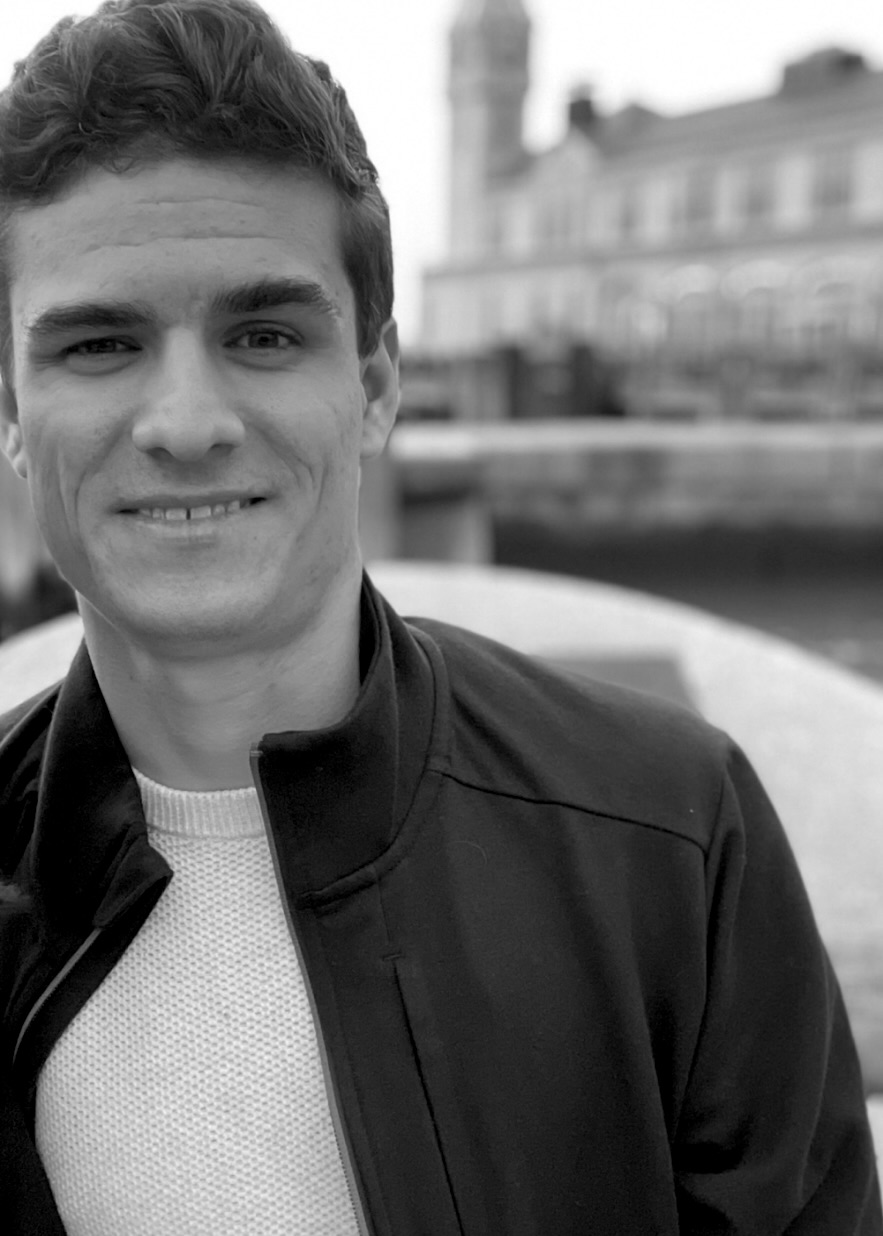
\includegraphics[height=1in]{img/paul.jpeg}
\end{wrapfigure}
\textbf{Paul Wood} is currently a senior at the University of Central Florida and will graduate with a Bachelor's of Science in Computer Engineering in May 2022. He is pursuing roles in low-level embedded systems, and is interested in operating systems and IoT devices. He plans on pursuing a graduate degree after working for a few years. \\

% Parke
\begin{wrapfigure}{l}{5em}
\centering
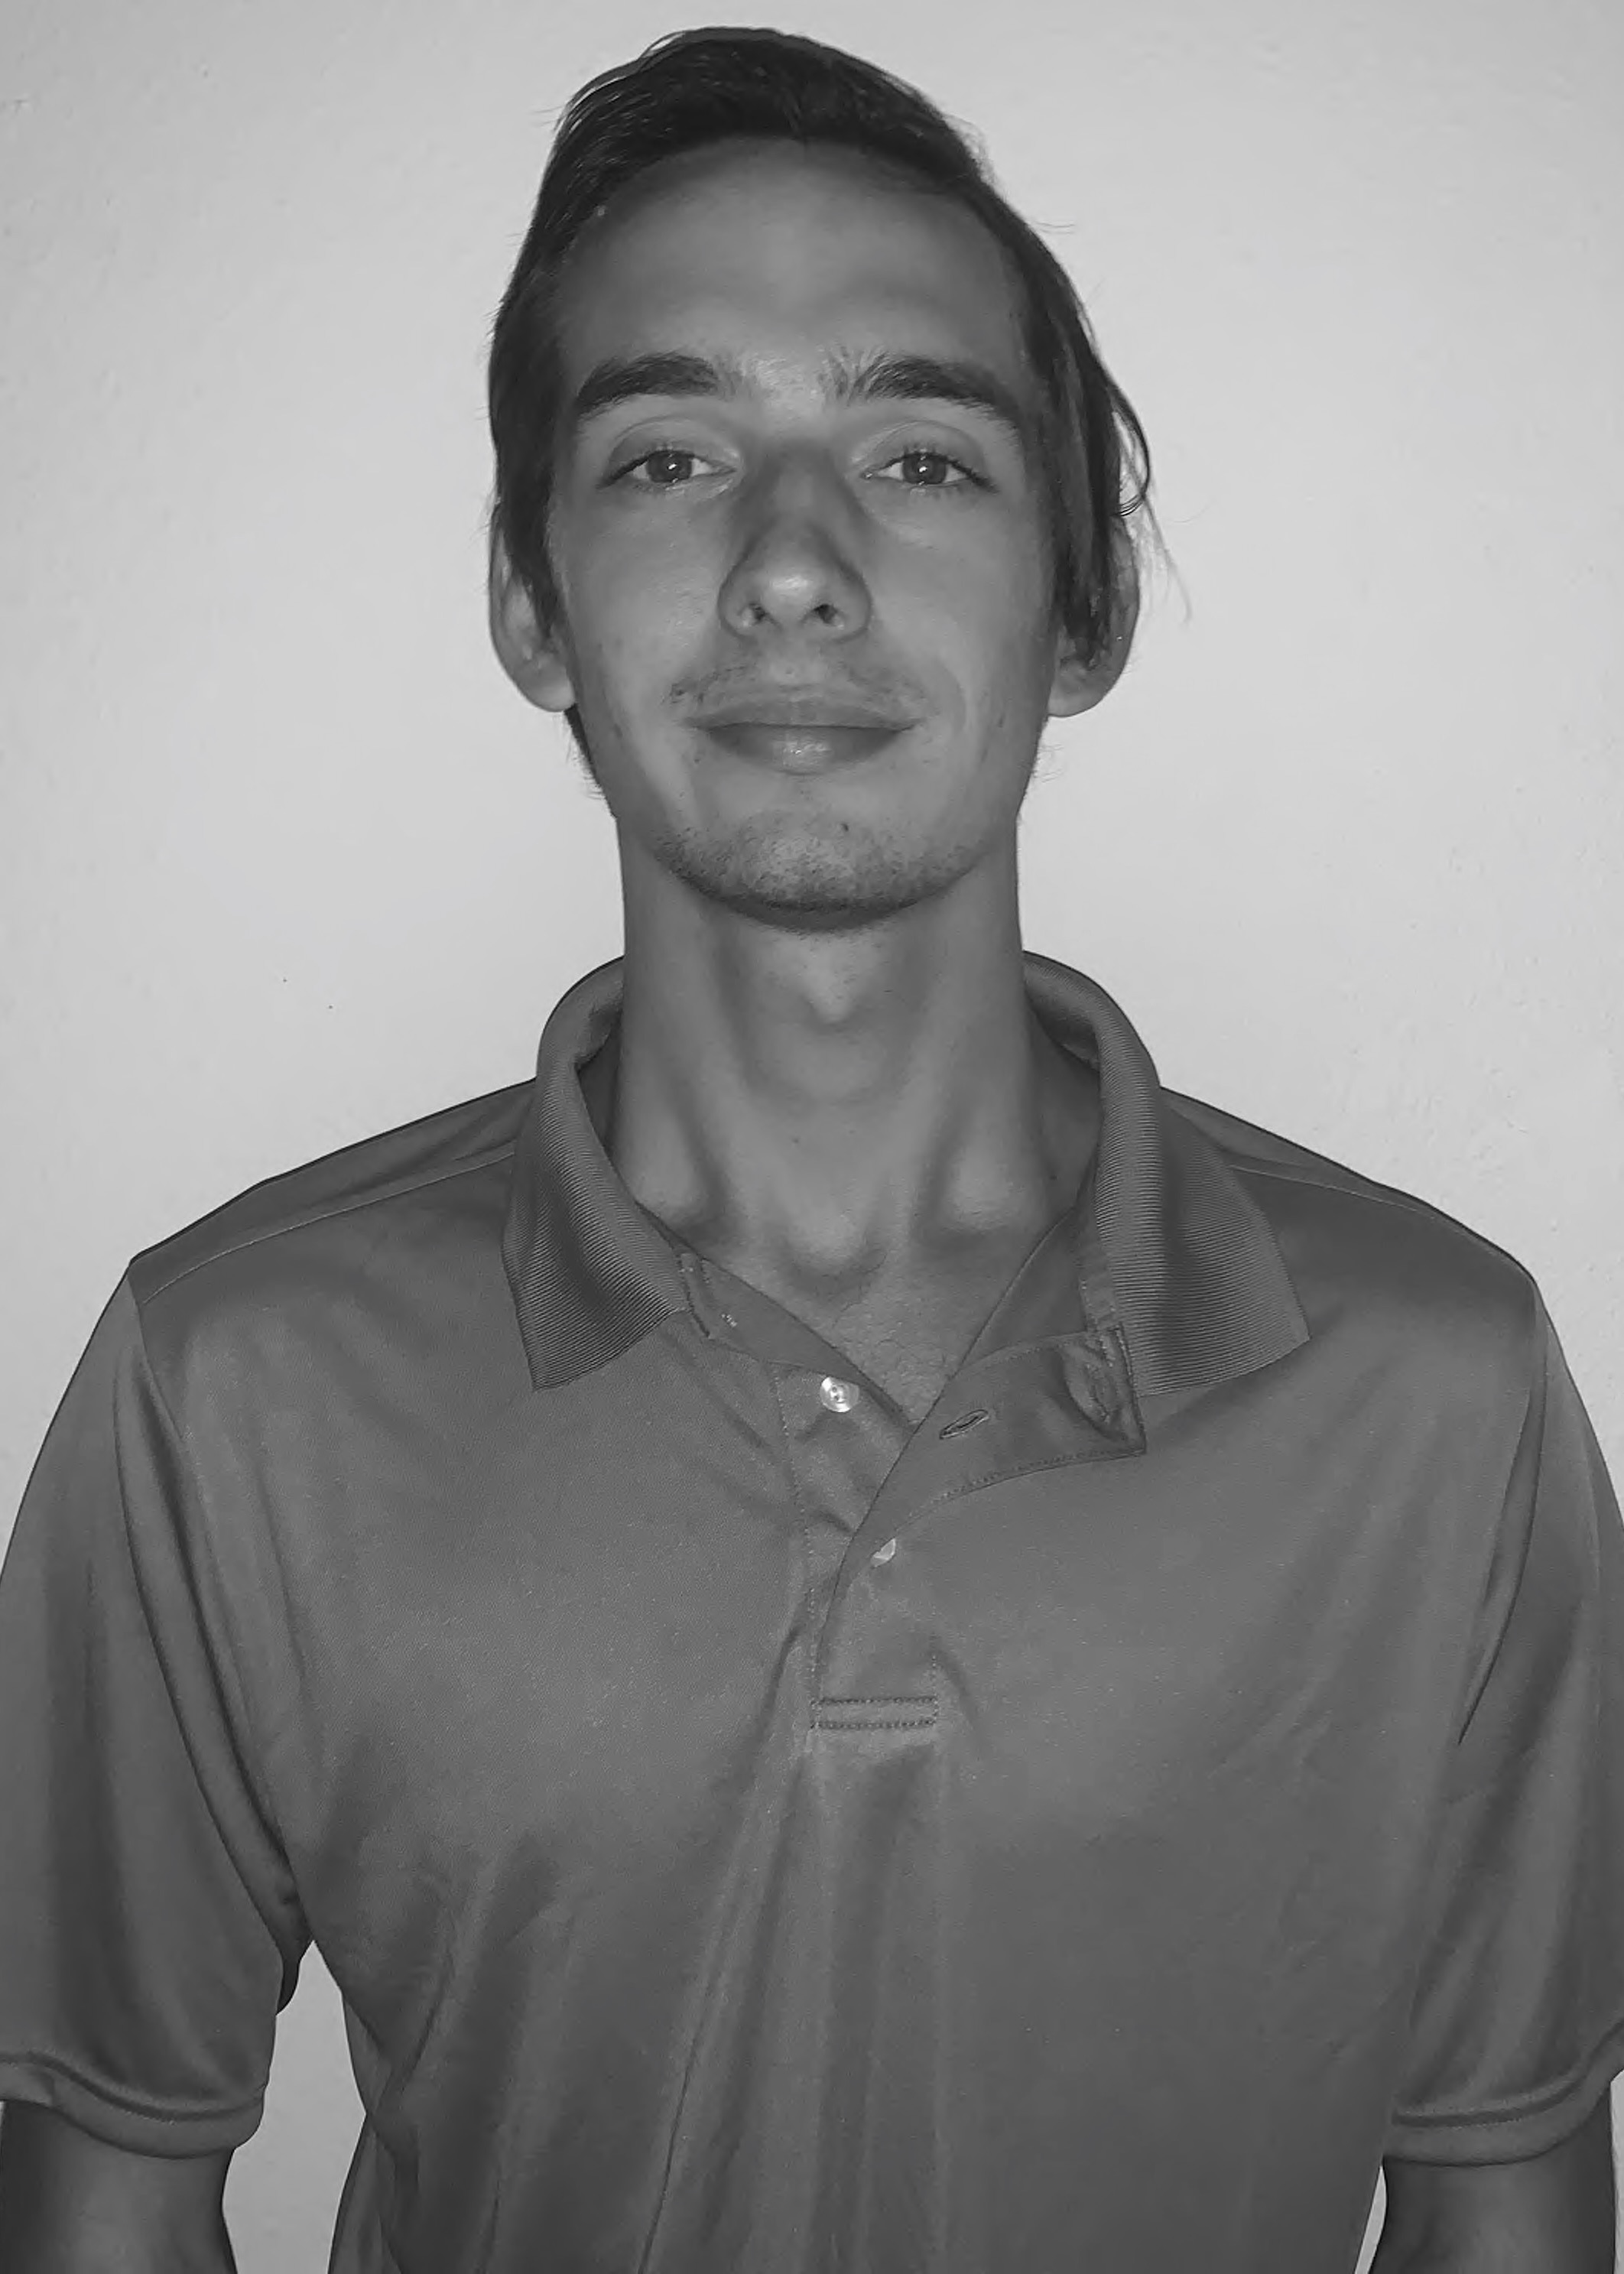
\includegraphics[height=1in]{img/Parke 2.jpeg}
\end{wrapfigure}
\textbf{Parke Benjamin} is currently a senior at the University of Central Florida and will graduate with a Bachelor's of Science in Electrical Engineering in May 2022. He is currently working at Duke Energy in Orlando, FL doing work in the protections and controls department. He plans on continuing to work there full-time, following his graduation. \\

% Randy
\begin{wrapfigure}{l}{5em}
\centering

\includegraphics[height=1in]{img/Randy.png}
\end{wrapfigure}
\textbf{Randy Alvarez} is currently a senior at the University of Central Florida and will graduate with a Bachelor's of Science in Electrical Engineering in May 2022. He is currently an intern in the CWEP program at Lockheed Martin in Orlando, FL doing work on systems testability and improvements. He plans on continuing to work there full-time, following his graduation. \\

\begin{thebibliography}{00}
\bibitem{background-aqi} Environmental Protection Agency, ``Technical assistance document for reporting of daily air quality,`` Available: https://www.airnow.gov/publications/air- quality-index/technical-assistance-document-for-reporting-the-daily-aqi/.

\bibitem{background-pm} Environmental Protection Agency, ``Health and environmental effects of particulate matter (pm),`` Available: https://www.epa.gov/pm-pollution/health-and-environmental- effects-particulate-matter-pm.

\bibitem{background-ozone} Environmental Protection Agency, ``Health effects of ozone in the general population,`` Available: https://www.epa.gov/ozone-pollution-and-your-patients-health/
health-effects-ozone-general-population.

\bibitem{bme688-datasheet} Bosch, ``Datasheet BME688: 4 in 1 Environmental Sensor with Artificial Intelligence,`` Available: https://media.digikey.com/pdf/Data\%20Sheets/Bosch/BST-BME688- \\ FL000-00.pdf

\bibitem{ZMOD4510-datasheet} Renesas, ``Datasheet ZMOD4510: Gas Sensor Modual for OAQ targeting NO2 & O3,`` Available: https://www.renesas.com/us/en/document/dst/zmod4510-datasheet

\bibitem{sps30-datasheet} Sensirion, ``Datasheet SPS30: Particulate Matter Sensor for Air Quality Monitoring and Control,`` Available: https://sensirion.com/media/documents/8600FF88/616542B5/Sensirion\_ \\
PM\_Sensors\_Datasheet\_SPS30.

\bibitem{MCP73871-datasheet} Microchip Technology, ``Datasheet MCP73871: Stand-Alone System Load Sharing and Li-Ion/Li-Polymer Battery Charge
Management Controller,`` Available: https://www.mouser.com/datasheet/2/268/MCP73871\_Data\_Sheet\_ \\
DS20002090F-2932254.pdf

% \bibitem{LTC3525-5-datasheet} Linear Technology, ``Datasheet LTC3525-5: Synchronous Step-Up DC/DC Converter with Output Disconnect,`` Available: https://www.mouser.com/datasheet/2/609/3525fc-1271864.pdf

% \bibitem{LP2985-datasheet} Texas Instruments, ``Datasheet LP2985:  Low-Noise, Low-Dropout Regulator With Shutdown,`` [Online] Available: https://www.ti.com/lit/ds/symlink/lp2985a.pdf?ts=1650392013905&ref\_ \\
% url=https\%253A\%252F\%252Fwww.google.com\%252F

\bibitem{cayenne} myDevicesIoT, ``Cayenne Low Power Payload,`` Available: https://github.com/myDevicesIoT/CayenneLPP

\end{thebibliography}

\end{document}
